% !TEX root =  ../main_iclr.tex



\begin{table}[h]%
\begin{minipage}[l]{0.4\textwidth}

\centering
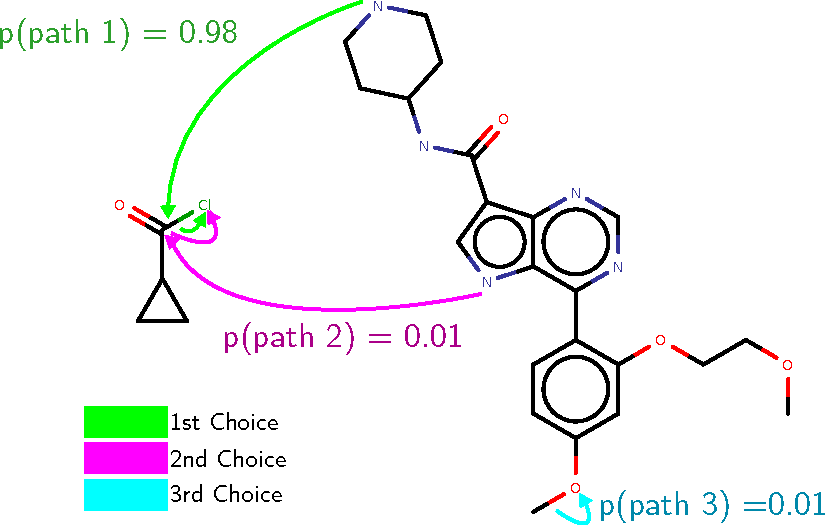
\includegraphics[width=1.\textwidth]{imgs/main_text_input}
\captionof{figure}{
An example of the paths suggested by \ourModelIR on one of the USPTO test examples. Its first choice in this instance is correct.
}
\label{fig:predicted-paths}
 \end{minipage}\hfill%
\begin{minipage}[r]{0.53\textwidth}
%  \centering
  \begin{tabular}{lllll}
    \toprule
    & \multicolumn{4}{c}{Accuracies (\%)}                   \\
    \cmidrule(r){2-5}
    Model Name & Top-1 & Top-2 & Top-3 & Top-5 \\
    \midrule
    \ourModelIR &  70.3 &  82.8 & 87.7 & 92.2    \\
    \ourModelR  &  77.8 &  89.2 & 92.4 & 94.7    \\
    \bottomrule
  \end{tabular}
  \caption{Results when using \ourModel for \emph{mechanism prediction}. Here a prediction is correct if the atom mapped action sequences predicted by our model match exactly those extracted from the USPTO dataset.}
  \label{table:mech-predict}
  \vspace{-0.25cm}
   \end{minipage}

\end{table}

We now evaluate \ourModelR on the task of (i) \emph{mechanism prediction} and (ii) \emph{product prediction} (as described in Figure~\ref{fig:task-overview}). While generally, it is necessary to know the reagents $\moleculeSet_e$ of a reaction to faithfully predict the mechanism and product, it is often possible to make inferences from the reactants alone. Therefore, we trained a second version of our model that we call \ourModelIR, which ignores reagent information. This allows us 
% when selecting the initial action (i.e.\ no context vector $\contextVect_\mathrm{reagent}$ is input into $\fInitial$), 
%allowing 
to gauge the importance of reagents in determining the mechanism of the reaction. %. We now evaluate our model on the \emph{reaction mechanism prediction} and \emph{reaction product prediction} problems.



% In our experiments we consider two variants of our model: 
% the first model \ourModelR  is exactly as defined in Section\ \ref{sec:model}, including all reagent information. 

% While generally all reagents are required to faithfully predict the mechanism and product, it is often possible to makes inferences from the reactants alone. Therefore, we investigated a second version we call \ourModelIR ignores the reagents when selecting the initial action (i.e.\ no context vector $\contextVect_\mathrm{reagent}$ is input into $\fInitial$), 
% allowing us to gauge the importance of reagents in determining what reaction occurs. We now evaluate our model on the \emph{reaction mechanism prediction} and \emph{reaction product prediction} problems.

\subsection{Reaction Mechanism Prediction}

For mechanism prediction we are interested in ensuring we obtain the exact sequence of electron steps correctly. 
%For instance, when forming a bond between two pairs of atoms we want to know which one of the atoms donated the electron pair needed to form the bond, even if the end result is the same. 
%The representation of the reaction mechanism produced by our model is a sequence of atoms, detailing the path taken by the electrons in a series of alternating steps in which bonds are broken and formed; using the atom mapping from the USPTO dataset this takes the form of a series of integers.
We evaluate accuracy by checking whether the sequence of integers extracted from the raw data as described in Section 4
is an exact match with the sequence of integers output by \ourModel. We compute the top-1, top-2, top-3, and top-5 accuracies and shown them in Table \ref{table:mech-predict}, with an example prediction shown in Figure \ref{fig:predicted-paths}.



\subsection{Reaction Product Prediction}
\label{sec:product-prediction}



\begin{table}[t]
%\begin{minipage}[l]{0.42\textwidth}
\begin{center}
	

 
  \label{table:prod-predict}
  %\end{minipage}\hfill
  %\begin{minipage}[r]{0.53\textwidth}
%  \centering
  \begin{tabular}{lllll}
    \toprule
    & \multicolumn{4}{c}{Accuracies (\%)}                   \\
    \cmidrule(r){2-5}
    Model Name & Top-1 & Top-2 & Top-3 & Top-5 \\
    \midrule
    WLDN FTS \citep{jin2017predicting} & 84.0  & 89.2 &  91.1 & 92.3 \\
    WLDN \citep{jin2017predicting} & 83.1 & 89.3 & 91.5 & 92.7 \\
    Seq2Seq FTS \citep{schwaller2017found} & 81.7 & 86.8 & 88.4 & 89.8 \\
    Seq2Seq \citep{schwaller2017found} & 82.6 & 87.3 & 88.8 & 90.1\\
    \bottomrule \toprule
    \ourModelIR &  78.2 & 87.7 & 91.5 & 94.4   \\
    \ourModelR  &  {\bf 87.0} & {\bf 92.6} & {\bf 94.5} & {\bf 95.9}    \\
    \bottomrule
  \end{tabular}
   \caption{Results for \emph{product prediction}, following the product matching procedure in Section~\ref{sec:product-prediction}. 
 For the baselines we compare against models trained (a) on the full USPTO training set (marked FTS) and only tested on our subset of LEF reactions, and (b) those that are also trained on the same subset as our model. 
 We make use of the code and pre-trained models provided by \citet{jin2017predicting}. For the Seq2Seq approach, as neither code nor more fine grained results are available, we train up the required models from scratch using the OpenNMT library \citep{2017opennmt}.
}
  %\end{minipage}
    \vspace{-0.25cm}
    \end{center}
\end{table}


Reaction mechanism prediction is useful for ensuring that we formed the correct product in the {\em correct way}.
However, this can underestimate the model's actual predictive accuracy: although a single atom mapping is provided as part of the USPTO dataset, in general atom mappings are not unique (e.g., if a molecule contains symmetries). Specifically, multiple different sequences of integers could correspond to chemically-identical electron paths. 
The first figure in the Appendix shows an example of a reaction with symmetries, where different electron paths produce the exact same product. 

Recent machine learning approaches to {\em product prediction} \citep{jin2017predicting,schwaller2017found}
have evaluated whether the major product reported in the test dataset matches predicted candidate products generated by their system, independent of mechanism.
In our case, the top-5 accuracy for a particular reaction may include multiple different electron paths that ultimately yield the same product molecule.

To evaluate if our model predicts the same major project as the one in the training data need to solve a graph isomorphism problem. To approximate this 
%Identifying whether two product molecules are chemically the same is equivalent to solving a graph isomorphism over the atoms and bond types, comparing the output of our system to the product molecule.
%To perform this comparison, 
we (a) take the predicted electron path, 
%sequence of edits on the reactants graph defined by an electron path,  
(b) apply these edits to the reactants to produce a product graph (balancing charge to satisfy valence constraints), 
(c) remove atom mappings,
and (d) convert the product graph to a canonical SMILES string representation in Kekul\'e form (aromatic bonds are explicitly represented as double-bonds). 
%then applying the sequence of edits to the reactants graph,
%setting explicit charges or hydrogen counts on the first and last atom in the electron path in order to satisfy valence constraints.
%We then strip all atom map numbers from the graph.
%We can use RDKit to express the molecule in a canonical SMILES string format 
%(predicted electron paths which yield chemically infeasible products are considered failures).
We can then evaluate whether a predicted electron path matches the ground truth by a string comparison. This procedure is inspired by the evaluation of \citet{schwaller2017found}. To obtain a ranked list of products for our model, we compute this canonicalized product SMILES for each of the predictions found by beam search over electron paths, removing duplicates along the way. 
These product-level accuracies are reported in Table~\ref{table:prod-predict}.

We compare with the state-of-the-art graph-based method \cite{jin2017predicting};
we use their evaluation code and pre-trained model\footnote{\url{https://github.com/wengong-jin/nips17-rexgen}},
re-evaluated on our extracted test set. 
We also use their code and re-train a model on our extracted training set, to ensure that any differences between our method and theirs is not due to a specialized training task. We also compare against the Seq2Seq model proposed by \citep{schwaller2017found}; 
however, as no code is provided by \citet{schwaller2017found}, we run our own implementation of this method based on the OpenNMT library \citep{2017opennmt}.
Overall, \ourModelR outperforms all other approaches on this task, with 87\% top-1 accuracy and 95.9\% top-5 accuracy.
Omitting the reagents in \ourModelR degrades top-1 accuracy slightly, but maintains a high top-3 and top-5 accuracy,
suggesting that reagent information is necessary to provide context in disambiguating plausible reaction paths.



% If the ultimate desired goal is to predict the product molecule rather than the reaction mechanism,
% a benefit of our approach is the predicted electron paths can then serve as an explanation. 
% In this manner, when showing predicted products, we can list, alongside the maximum likelihood path, any other candidate paths that result in the same product. 




